%%%%%%%%%%%%%%%%%%%%%%%%%%%%%%%%%%%%%%%%%%%%%%%%%%%%%%%%%%%%
\documentclass[xcolor=x11names,compress]{beamer}

\definecolor{CoolBlack}{rgb}{0.0, 0.18, 0.39}
\definecolor{byellow}{rgb}{0.55037, 0.38821, 0.06142}
%% General document %%%%%%%%%%%%%%%%%%%%%%%%%%%%%%%%%%
\usepackage{graphicx}
\usepackage{tikz}
\usetikzlibrary{decorations.fractals}
%%%%%%%%%%%%%%%%%%%%%%%%%%%%%%%%%%%%%%%%%%%%%%%%%%%%%%

%% Beamer Layout %%%%%%%%%%%%%%%%%%%%%%%%%%%%%%%%%%
\useoutertheme[subsection=false,shadow]{miniframes}
\useinnertheme{default}
\usefonttheme{serif}
\usepackage{palatino}
\usepackage{tabu}

% addition of color
\usepackage{xcolor}
\definecolor{dgreen}{rgb}{0.,0.6,0.}
\definecolor{RawSienna}{cmyk}{0,0.72,1,0.45}

\setbeamerfont{title like}{shape=\scshape}
\setbeamerfont{frametitle}{shape=\scshape}

\setbeamercolor*{lower separation line head}{bg=CoolBlack} 
\setbeamercolor*{normal text}{fg=black,bg=white} 
\setbeamercolor*{alerted text}{fg=red} 
\setbeamercolor*{example text}{fg=black} 
\setbeamercolor*{structure}{fg=black} 
 
\setbeamercolor*{palette tertiary}{fg=black,bg=black!10} 
\setbeamercolor*{palette quaternary}{fg=black,bg=black!10} 

\renewcommand{\(}{\begin{columns}}
\renewcommand{\)}{\end{columns}}
\newcommand{\<}[1]{\begin{column}{#1}}
\renewcommand{\>}{\end{column}}

% adding slide numbers
\addtobeamertemplate{navigation symbols}{}{%
    \usebeamerfont{footline}%
    \usebeamercolor[fg]{footline}%
    \hspace{1em}%
    \insertframenumber/\inserttotalframenumber
}

% equation stuff
\newcommand{\Macro}{\ensuremath{\Sigma}}
\newcommand{\Sn}{\ensuremath{S_N} }
\newcommand{\vOmega}{\ensuremath{\hat{\Omega}}}
\usepackage{mathrsfs}
\usepackage[mathcal]{euscript}
\usepackage{amssymb}
\usepackage{amsthm}
\usepackage{epsfig}
\usepackage{amsmath}

\newcommand{\ve}[1]{\ensuremath{\mathbf{#1}}}
\newcommand{\micro}{\ensuremath{\sigma}}
\newcommand{\detR}{\ensuremath{\Sigma}}
%%%%%%%%%%%%%%%%%%%%%%%%%%%%%%%%%%%%%%%%%%%%%%%%%%

\begin{document}

%%%%%%%%%%%%%%%%%%%%%%%%%%%%%%%%%%%%%%%%%%%%%%%%%%%%%%
%%%%%%%%%%%%%%%%%%%%%%%%%%%%%%%%%%%%%%%%%%%%%%%%%%%%%%
\begin{frame}
\title{Recent Past and Planned Research}
\subtitle{Reactor Design and Neutronics Group}
\author{
        \includegraphics[height=2cm]{bk}\\R.\ N.\ Slaybaugh}

\date{April 15, 2014}
\titlepage
\end{frame}

% --------------------------------------------------------------
\begin{frame}[fragile]{Outline}
  \frametitle{Outline}
  \begin{itemize}
    \item Hybrid methods overview
    \begin{itemize}
     	\item Motivation
		\item CADIS
		\item FW-CADIS
		\item Challenges
    \end{itemize}
	\item MC importances in the presence of space and energy self-shielding
	\begin{itemize}
    		\item Cross Section Processing
		\item Problem Investigation
		\item Resonance Factor Method
		\item Results
		\item Summary and Conclusions
  	\end{itemize}
	\item MC importances for problems with strong anisotropies
	\item Other potential projects
  \end{itemize}

\end{frame}


% --------------------------------------------------------------
% --------------------------------------------------------------
\section{\scshape Hybrid Methods}
\subsection{Motivation}
\begin{frame}[fragile]
  \frametitle{Solving the TE}

\begin{columns}
  \begin{column}{0.5\textwidth}
  \begin{center}
  \underline{Monte Carlo}
  \end{center}
	\begin{itemize}
	\item Solution has associated statistical error
	\item Continuous phase space: ``gold standard answers"
	\item Can take a long time
	\item Good for streaming
	\item Optically thick = slow
	\end{itemize}
  \end{column}
  \begin{column}{0.5\textwidth}
  \begin{center}
  \underline{Deterministic}
  \end{center}
	\begin{itemize}
	\item Solution equally valid everywhere
	\item Discretized phase space: drives solution quality
	\item Can be fast
	\item Streaming = ray effects
	\item Good for optically thick
	\end{itemize}
  \end{column}
\end{columns}

\end{frame}

% --------------------------------------------------------------
\begin{frame}[fragile]
  \frametitle{Acceleration}
  \begin{itemize}
  	\item To use MC in many applications, we need to \textit{accelerate} it
	\item Variance reduction is designed to improve the FOM:
  \end{itemize}
\begin{align}
\text{FOM} = \frac{1}{\text{R}^2\text{t}} \qquad & \text{R = relative error} \nonumber \\ 
& \text{t = time} \nonumber 
\end{align}
  \begin{itemize}
  	\item \underline{Idea}: can we use deterministic and Monte Carlo methods together to lessen the weaknesses of each?
  \end{itemize}
  $\rightarrow$ \textbf{Hybrid Methods}

\end{frame}


% --------------------------------------------------------------
\subsection{CADIS}
\begin{frame}[fragile]
  \frametitle{CADIS}
Define response with function $f(\ve{r}, E)$ in volume, $V_d$ as
%
\begin{equation}
 R = \int_E \int_{V_f} f(\ve{r}, E) \phi(\ve{r}, E) dV dE 
 \label{eq:Response}
\end{equation}
%
\begin{columns}
  \begin{column}{0.5\textwidth}
	\begin{align}
  	H\phi &= q \quad \text{(forward)}\nonumber \\
  	%
  	H^{\dagger} \phi^{\dagger} &= q^{\dagger} \quad 
  	\text{(adjoint)}\nonumber
  	\end{align}
  \end{column}
  \begin{column}{0.5\textwidth}
  	\begin{align}
  	\langle H\phi, \phi^{\dagger} \rangle &= \langle H^{\dagger} \phi^{\dagger}, \phi \rangle \:, \text{and therefore} \nonumber \\
  	%
  	\langle q, \phi^{\dagger} \rangle &= \langle q^{\dagger}, \phi \rangle \nonumber
  	\end{align}
  \end{column}
\end{columns}
\vspace*{1 em}
If we let $q^{\dagger} = f(\ve{r}, E)$ then
%
\begin{equation}
 \langle q^{\dagger}, \phi \rangle = \langle f, \phi \rangle = R = \langle q, \phi^{\dagger} \rangle
 \label{eq:ResponseRedef}
\end{equation}
%
Eq.\ \eqref{eq:ResponseRedef} expresses that $\phi^{\dagger}$ represents the expected contribution of a source particle to the response given the source, $q$.

\end{frame}

% --------------------------------------------------------------
\begin{frame}[fragile]
  \frametitle{CADIS}
  
  \begin{enumerate}
  \item Define $q^{\dagger}$ as the local response of interest\\
  \item Generate $\phi^{\dagger}$ and $R$ with a coarse deterministic solution
  \end{enumerate}
% 
\begin{align}
  imp(\ve{r}, E) &= \frac{\phi^{\dagger}(\ve{r}, E)}{\langle q(\ve{r}, E), \phi^{\dagger}(\ve{r}, E) \rangle} = \frac{\phi^{\dagger}(\ve{r}, E)}{R(\ve{r}, E)} \\
  %
  \hat{q}(\ve{r}, E) &= \frac{\phi^{\dagger}(\ve{r}, E) q(\ve{r}, E)}{R} \\
  %
  w_0(\ve{r}, E) &= \frac{q(\ve{r}, E)}{\hat{q}(\ve{r}, E)} = \frac{R}{\phi^{\dagger}(\ve{r}, E)} 
  \label{eq:Importance}
\end{align}

Birth weights match weight targets, making this the \underline{C}onsistent \underline{A}djoint \underline{D}riven \underline{I}mportance \underline{S}ampling \underline{M}ethod

\end{frame}

% --------------------------------------------------------------
\subsection{FW-CADIS}
\begin{frame}[fragile]
  \frametitle{FW-CADIS}

\begin{itemize}
\item We often what to optimize solutions in all of phase space\\
\item In this case the adjoint source needs to be a global forward solution: \underline{F}orward \underline{W}eighted-CADIS
\end{itemize}
%
\begin{columns}
  \begin{column}{0.5\textwidth}
  \begin{center}
  \textcolor{byellow}{To Optimize}
  \end{center}
	\begin{align}
  	&\phi(\ve{r}, E)\nonumber \\
  	%
  	\int&\phi(\ve{r}, E)\sigma_d(\ve{r}, E)\nonumber
  	\end{align}
  \end{column}
  %
  \begin{column}{0.5\textwidth}
  \begin{center}
  \textcolor{byellow}{Adjoint Source}
  \end{center}
  	\begin{align}
  	f(\ve{r}, E) &= \frac{1}{\phi(\ve{r}, E)}\nonumber \\
  	%
  	f(\ve{r}, E) &= \frac{\sigma_d(\ve{r}, E)}{\int\phi(\ve{r}, E)\sigma_d(\ve{r}, E)} \nonumber
  	\end{align}
  \end{column}
\end{columns}
\vspace*{1 em}
For example
%
\begin{equation}
 R = \int_E \int_{V_f} f(\ve{r}, E) \phi(\ve{r}, E) dV dE = \int_E \int_{V} \frac{1}{\phi(\ve{r}, E)} \phi(\ve{r}, E) dV dE \approx 1 \nonumber
\end{equation}

\end{frame}

% --------------------------------------------------------------
\subsection{Challenges}
\begin{frame}[fragile]
  \frametitle{Challenges}

	FW-CADIS works well for \textbf{most} deep penetration
	shielding problems...
	%
	\begin{columns}
  	\begin{column}{0.5\textwidth}
  	\begin{figure}
  	\begin{center}
  		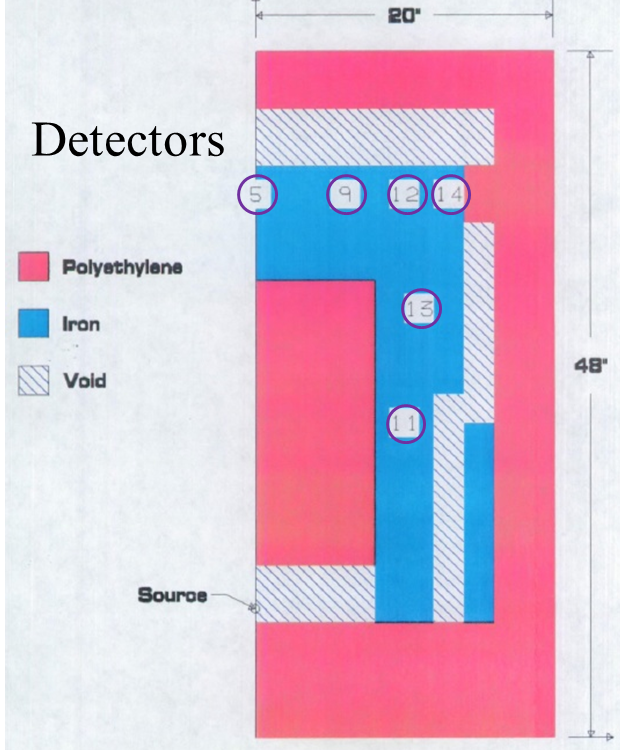
\includegraphics[height=2in,clip]{dlvn}
		\caption{Dog Legged Void Neutron Shielding Benchmark}
	\end{center}
  	\end{figure}
  	\end{column}
 	%
 	\begin{column}{0.5\textwidth}
 	\begin{figure}
  	\begin{center}
  		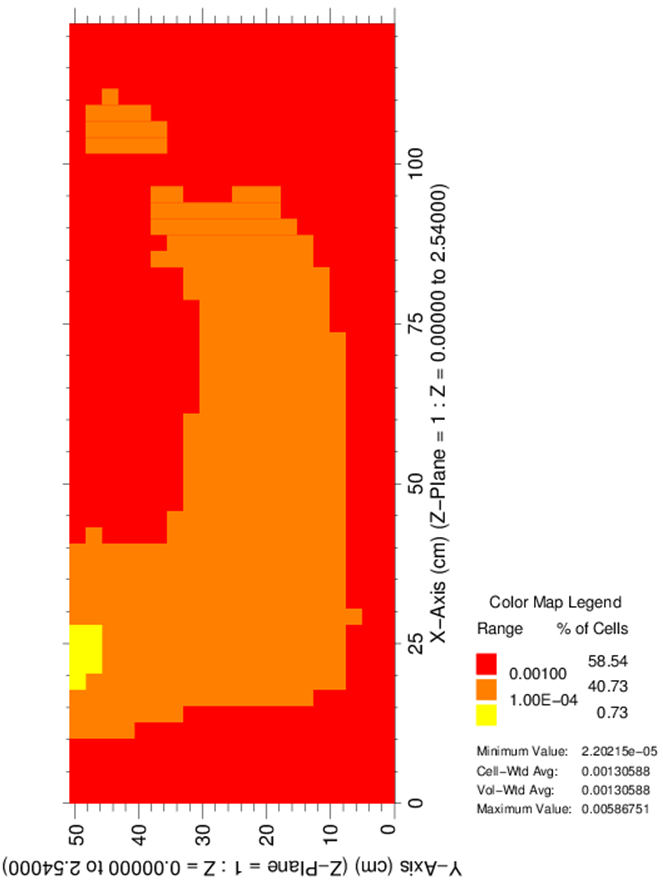
\includegraphics[height=2in,clip]{dlvn-lowVR}
  		\caption{MC 95\% CI RE using FW-CADIS, DLVN}
  	\end{center}
  	\end{figure}
  	\end{column}
	\end{columns}
  
\end{frame}

% --------------------------------------------------------------
\begin{frame}[fragile]
  \frametitle{Challenges}

	...but not all of them
	%
	\begin{columns}
  	\begin{column}{0.5\textwidth}
  	\begin{center}
		\begin{itemize}
		\item FW-CADIS only includes space and energy, 
			\textit{not angle}
		\item One pathological case:
		\begin{itemize}
		\item Energy self-shielding +
		\item Spatial self-shielding
		\end{itemize}
		\item High relative error through location of Interest
		\item Outcome: new methods based on FW-CADIS
		\item The Resonance Factor method uses different cross section processing
		\end{itemize}
	\end{center}
  	\end{column}
 	%
 	\begin{column}{0.5\textwidth}
  	\begin{center}
  	\begin{figure}
  		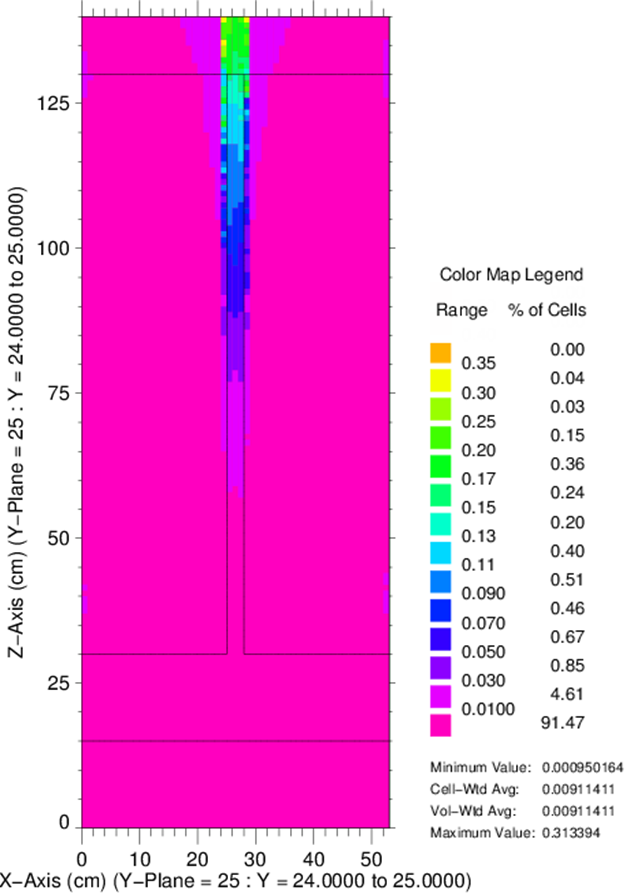
\includegraphics[height=2in,clip]{plate-badVR}
  		\caption{MC 95\% CI RE using FW-CADIS, Plate}
  	\end{figure}
  	\end{center}
  	\end{column}
	\end{columns}
  
\end{frame}


% --------------------------------------------------------------
% --------------------------------------------------------------
\section{Self-Shielding}
\subsection{Cross Section Processing}
\begin{frame}[fragile]
  \frametitle{Cross Section Processing}

	\begin{itemize}
	\item General Case
	\begin{equation}
  	\micro_{x,g}^{(j)} = \frac{\langle \micro_x^{(j)}(u) W(u)\rangle}
	{\langle W(u)\rangle} \:, \quad W(u) = \phi_{\infty}(u)
 	 \label{eq:baseBondarenko}
 	\end{equation} 
 	
 	\item Bondarekno method uses a background cross section
 	\begin{equation}
  	\micro_0^{(j)} = \frac{1}{N_j} \sum_{m \ne j} \micro_{t}^{(m)} N_m 
  	%\label{eq:bgxsec}
  	\:, \quad \micro_{x,g}^{(j)}(\micro_0^{(j)}y) = \frac{\langle
  	 \micro_{x}^{(j)}(u) \frac{\phi_{\infty}(u)} {\micro_{t}^{(j)}(u)
  	 + \micro_0^{(j)}} \rangle}
  	 { \langle \frac{\phi_{\infty}(u)}{\micro_{t}^{(j)}(u) +
  	 \micro_0^{(j)}}\rangle}
  \label{eq:ssfact}
	\end{equation}

	\item W(u) changed to include the  spectral difference assumption and effect of other isotopes
	\end{itemize}
	
\end{frame}
	
% --------------------------------------------------------------
\begin{frame}[fragile]
  \frametitle{Cross Section Processing}

	\begin{itemize}
	\item When When a nuclide is dilute, $\sigma_0^{(j)} >>
	 \sigma_t^{(j)}$, \\$W(u) \rightarrow$ uncorrected 
		\begin{itemize}
		\item Large $\sigma_0$ = infinitely dilute case	
		\end{itemize}

	\item When a nuclide is concentrated, $\sigma_0^{(j)} << 
	 \sigma_t^{(j)}$, resonances have a larger impact 
		\begin{itemize}
		\item Small $\sigma_0$ = resonance case	
		\end{itemize}
	\end{itemize}
	
	\begin{itemize}
	\item Add correction for `thin slab' of resonance material in 
	`thick slab' of moderator
	\begin{align}
  	&\sigma_0^{*,(j)} = \frac{1}{N_j} \sum_{m \ne j} \sigma_{t}^{(m)} N_m 
	+ \frac{1}{N_j \bar{l}} \\
  	&\text{\textcolor{byellow}{thin slab:}}\:\bar{l} \approx \frac{4V}{S} \qquad \text{\textcolor{byellow}{no effect:}}\:\bar{l} \approx \text{large} \nonumber
	\end{align}
	\end{itemize}
  
\end{frame}

% --------------------------------------------------------------
\subsection{Problem Investigation}
\begin{frame}[fragile]
  \frametitle{Problem Investigation}
  	\begin{columns}
  	\begin{column}{0.45\textwidth}
  	\begin{figure}
  		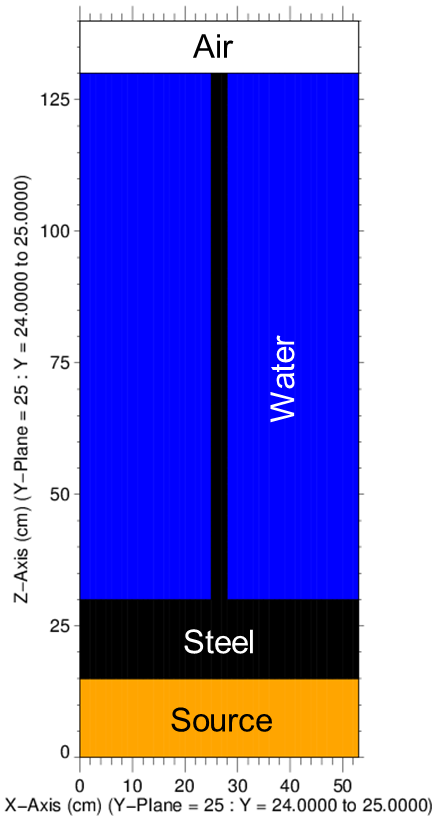
\includegraphics[height=2in,clip]{plate-geometry}
  		\caption{Shielding Stack Up}
  	\end{figure}
  	\end{column}
 	%
 	\begin{column}{0.6\textwidth}
	\begin{itemize}
	\item 53 cm $\times$ 50 cm $\times$ 140 cm 
	\item Uniform in x except plate (25-28 cm in x; 30-130 cm in z)
	\item Uniform in y
	\item U-235 fission spectrum; homogenized U, Zr, and H2O
	\vspace*{1 em}
	\item MC21, MCNP, and PARTISN
	\item ENDF/B-VII data (all codes)
	\item Processed by TRANSX (multigroup)
	\end{itemize}
  	\end{column}
	\end{columns}
  
\end{frame}


% --------------------------------------------------------------
\begin{frame}[fragile]
  \frametitle{Base Calculation Parameters}
  \begin{table}[p]
  \label{tab:calcParams}
  \begin{center}
    \begin{tabu}{| X | X | X |}\hline
      Variable & PARTISN & MC21\\\hline\hline
	Deterministic Mesh & 0.5 cm unif; 0.25 cm in $x$ over 24 to 29 cm & 1 cm uniform \\\hline
	Tally mesh & N/A & 1 cm uniform \\\hline
	N particles & N/A & $1 \times 10^{10}$\\\hline
	Energy structure & 58 grps & 27 grps / continuous\\\hline
	Angular quad & QR-18-252 & QR-8-36\\\hline
	Scattering order & $P_3$ & $P_3$\\\hline
	Convergence & 0.01 & 0.05\\\hline
	TRANSX settings & default & default\\\hline
	DCFs & 58 grps & 27 grps \\\hline
    \end{tabu}
  \end{center}
\end{table}
  
\end{frame}

% --------------------------------------------------------------
\begin{frame}[fragile]
  \frametitle{Errors in Plate}
 \begin{figure}[p]
   \begin{center}
     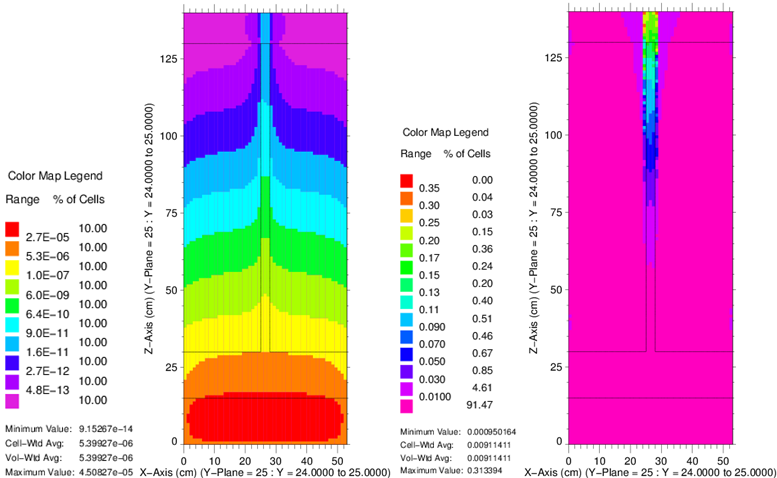
\includegraphics[height=2 in,clip]{NSE13-109R1-PlateDRandRE}
   \end{center}
   \caption{Plate base FW-CADIS MC21 dose rate (left) and 95CI RE (right) (xz-slice through y=25 cm)}
   \label{fig:Plate}
 \end{figure}
\end{frame}

% --------------------------------------------------------------
\begin{frame}[fragile]
  \frametitle{Deterministic MC Mismatch}
 \begin{figure}[p]
   \begin{center}
     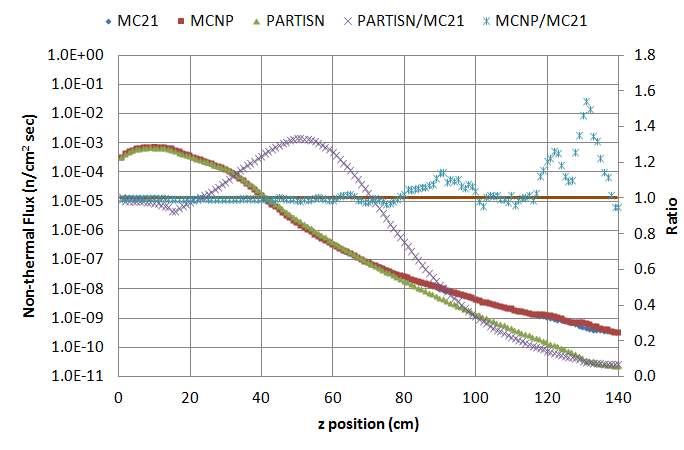
\includegraphics[width=4in,clip]{NSE13-109R1-PlateFluxExcel}
   \end{center}
   \caption{Plate non-thermal flux (left axis) and method ratios (right axis) down the x-y centerline}
   \label{fig:PlateFlux}
 \end{figure}
\end{frame}

% --------------------------------------------------------------
\begin{frame}[fragile]
  \frametitle{Deterministic MC Mismatch}
 \begin{figure}[p]
   \begin{center}
     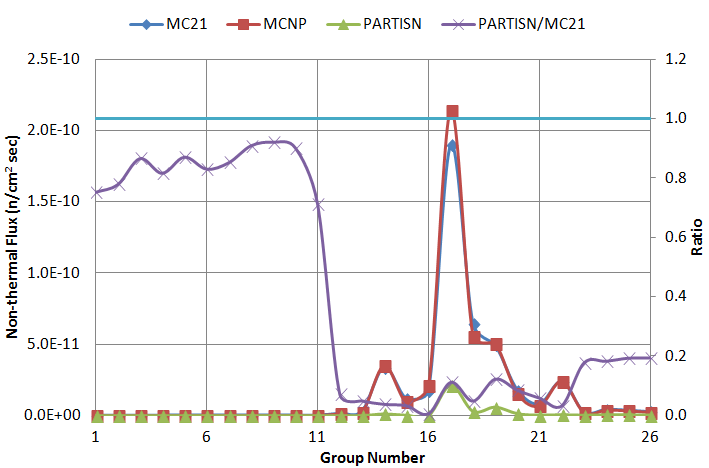
\includegraphics[width=4in,clip]{NSE13-109R1-PlateExitSpectra}
   \end{center}
   \caption{Plate flux spectra (left axis) and PARTSN/MC21 (right axis) at start of air region (z = 130.5 cm)}
   \label{fig:PlateExit}
 \end{figure}
\end{frame}

% --------------------------------------------------------------
\begin{frame}[fragile]
  \frametitle{Correct Without Plate}
 \begin{figure}[p]
   \begin{center}
     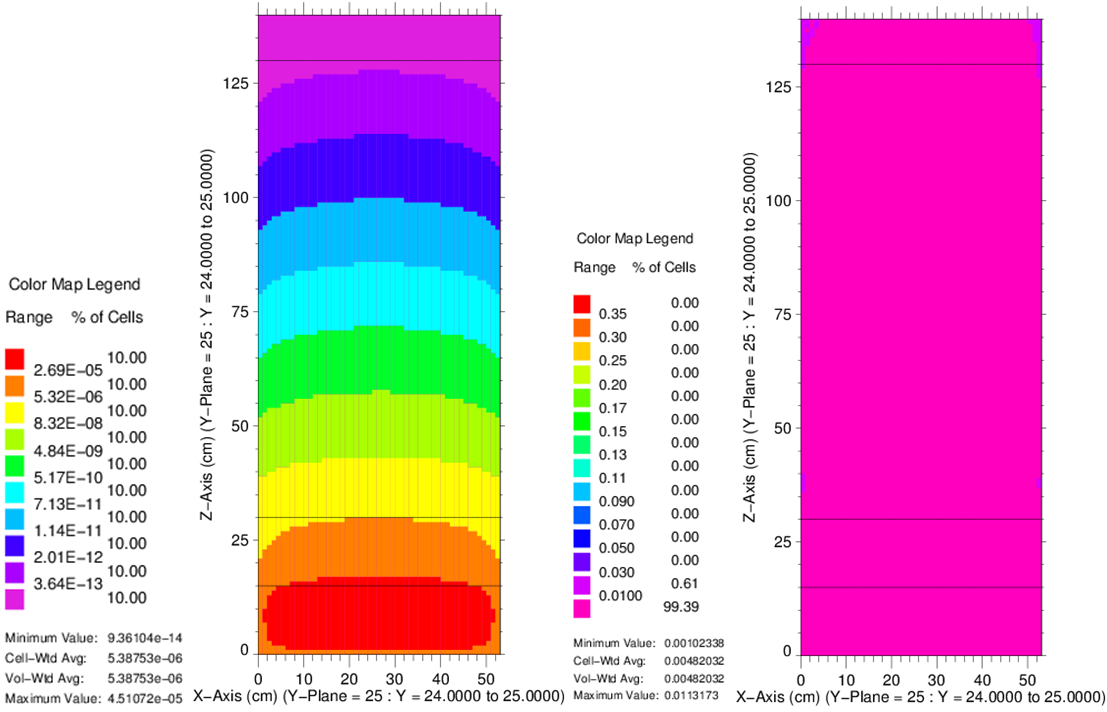
\includegraphics[height=2in,clip]{NSE13-109R1-NoPlateDRandRE}
   \end{center}
   \caption{No-Plate MC21 dose rate (left) and 95CI RE (right) (xz-slice through y=25 cm)}
   \label{fig:noPlate}
 \end{figure}
\end{frame}

% --------------------------------------------------------------
\begin{frame}[fragile]
  \frametitle{Correct Without Plate}
 \begin{figure}[p]
   \begin{center}
     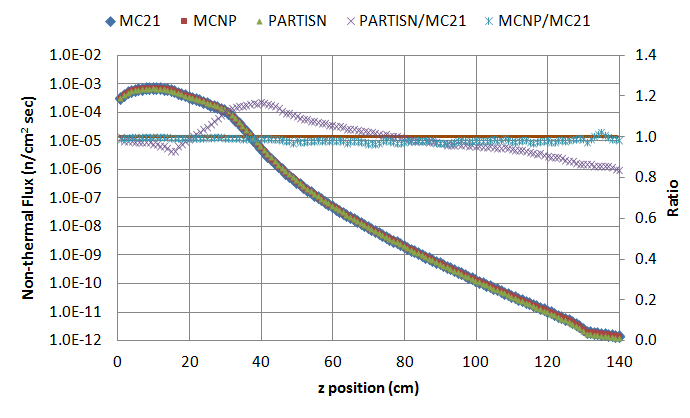
\includegraphics[width=4in,clip]{NSE13-109R1-NoPlateFluxExcel}
   \end{center}
   \caption{Plate non-thermal flux (left axis) and method ratios (right axis) down the x-y centerline}
   \label{fig:noPlateFlux}
 \end{figure}
\end{frame}

% --------------------------------------------------------------
\subsection{Resonance Factor Method}
\begin{frame}[fragile]
  \frametitle{Resonance Factor Method}
  
\end{frame}


% --------------------------------------------------------------
\subsection{Results}
\begin{frame}[fragile]
  \frametitle{Results}
  
\end{frame}


% --------------------------------------------------------------
\subsection{Summary and Conclusions}
\begin{frame}[fragile]
  \frametitle{Summary and Conclusions}
  
\end{frame}

% --------------------------------------------------------------
% --------------------------------------------------------------
\section{Strong Anisotropies}
\begin{frame}[fragile]
  \frametitle{}

  
\end{frame}


% --------------------------------------------------------------
% --------------------------------------------------------------
\section{Other Potential Projects}
\begin{frame}[fragile]
  \frametitle{}

  
\end{frame}


% --------------------------------------------------------------
% --------------------------------------------------------------
\section*{}
\begin{frame}[fragile]
  \frametitle{Questions?}
  \begin{center}
  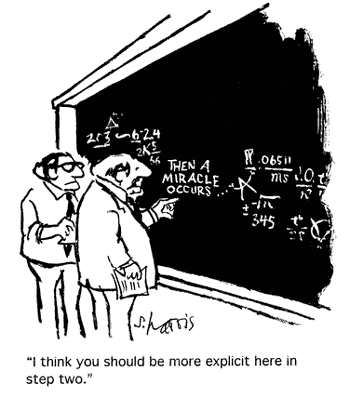
\includegraphics[height=3in,clip]{../questions-comic}  
  \end{center}
  
\end{frame}

% --------------------------------------------------------------
\section*{}
\begin{frame}[fragile]
	\begin{columns}
  	\begin{column}{0.5\textwidth}

  	\end{column}
 	%
 	\begin{column}{0.5\textwidth}


  	\end{column}
	\end{columns}
	
  	\begin{center}
  	\begin{figure}
  		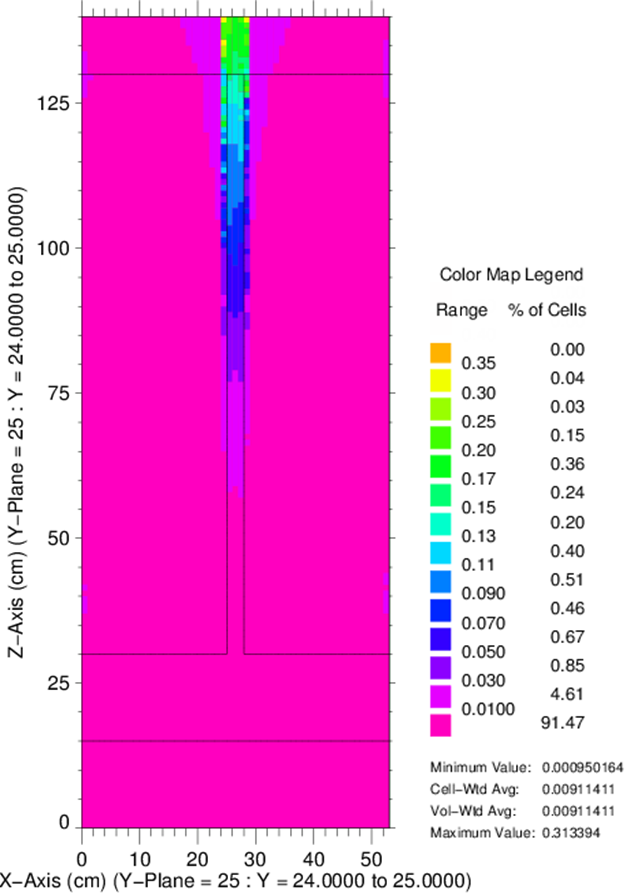
\includegraphics[height=2in,clip]{plate-badVR}
  		\caption{MC 95\% CI RE using FW-CADIS, Plate}
  	\end{figure}
  	\end{center}
  
\end{frame}


\end{document}